\section{Variational Autoencoders}

  Note that like linear latent variable models such as PCA, autoencoders ``encode'' our samples in a latent space, which we will call $\mathcal{Z}$. If we wanted to create a generative model from autoencoders, we can use the analogous transition from PCA to PPCA, by changing our points to distributions. Like in PPCA, we might want to define a standard Gaussian over the latent space $\mathcal{Z}$ and transform this into the original space $\mathcal{X}$. However, there is a small problem with autoencoders. The latent space where the encoded vectors lie may not be contiguous, which means that the distribution of the latent space may not be very simple either. Look at the encodings of MNIST below. Trying to sample from this space with a isotropic Gaussian results in a high probability of hitting the ``dead'' zones which may give garbage generative results. If the space has discontinuities and you sample a variation from there, the decoder will simply generate an unrealistic output. 

  \begin{figure}[H]
    \centering
    \begin{subfigure}[b]{0.48\textwidth}
      \centering
      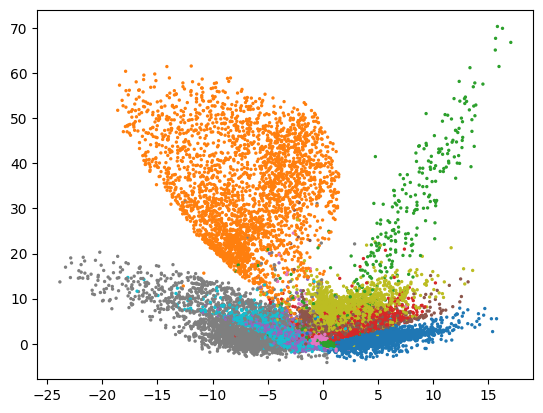
\includegraphics[scale=0.36]{img/08_VAE/mnist_latent.png}
      \caption{Training an autoencoder on MNIST and then visualizing the encodings from a 2D latent space shows the formation of distinct clusters, but there are huge empty spaces where the labeling may be ambiguous and not allow us to interpolate effectively. }
      \label{fig:mnist_latent}
    \end{subfigure}
    \hfill 
    \begin{subfigure}[b]{0.48\textwidth}
      \centering
      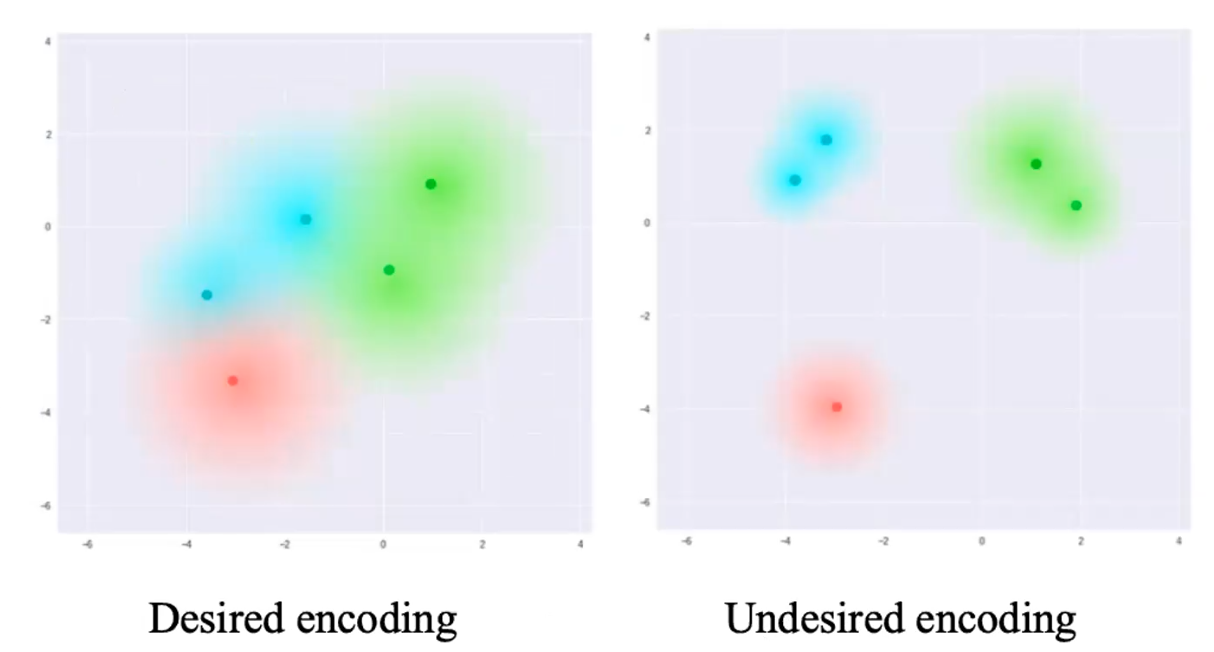
\includegraphics[scale=0.22]{img/08_VAE/contiguous_encoding.png}
      \caption{ Therefore, we want the encodings to be contiguous while still being distinct. This allows smooth interpolation which is easy to sample from with a simple pdf, e.g. Gaussian, and enables construction of \textit{new} samples. } 
      \label{fig:contiguous_encoding}
    \end{subfigure}
    \caption{}
    \label{fig:motivation_vae}
  \end{figure}

  In 2013, Kigma introduced this generative model that bridges between latent variable models and deep neural nets. 

  In a classification neural network, it takes in an input $\mathbf{x}$ and outputs a softmax vector $NN(\mathbf{x}) =(p_1, \ldots, p_K)^T$. This basically means that $NN(\mathbf{x}) = \boldsymbol{\theta}$ parameterizes the conditional distribution (in this case, multinomial) of $\mathbf{y}$ given $\mathbf{x}$. 
  \begin{equation}
    Y \mid X = x \sim \mathrm{Multinomial}(\boldsymbol{\theta} = NN(\mathbf{x}))
  \end{equation}
  This is a much more efficient way to store conditional distributions than a $\dim(X) (K - 1)$ lookup table. 

  \subsection{Deep Latent Variable Models}

    Latent variable models that uses some deep learning architecture is pretty much what DLVMs are. This is essentially what we want to extend. We take a latent model $(\mathbf{x}, \mathbf{z})$ and want to approximate $p(\mathbf{x}, \mathbf{z})$. There are essentially 2 things we're interested in: 
    \begin{enumerate}
        \item \textbf{Generation}: Computing $p(\mathbf{x} \mid \mathbf{z})$. 
        \item \textbf{Inference}: Computing $p(\mathbf{z} \mid \mathbf{x})$. 
    \end{enumerate}
    Given a latent sample $\mathbf{z}$ we want to find the conditional probability distribution of $\mathbf{x}$ given $\mathbf{z}$. We can also assume a simple prior $p(\mathbf{z})$ and calculate 
    \[p(\mathbf{x}, \mathbf{z}) = p(\mathbf{x} \mid \mathbf{z}) \, p(\mathbf{z}) \]
    That is, we generate a latent variable from $p(\mathbf{z})$ and want to use this value to get the parameters of $x \sim p_{\boldsymbol{\theta}} (\mathbf{x} \mid \mathbf{z})$ with some decoder neural network $D_{\boldsymbol{\theta}}$ that parameterizes the distribution. Clearly put, $D_{\boldsymbol{\theta}} (\mathbf{z})$ are the parameters of $\mathbf{X} \mid \mathbf{Z} = \mathbf{z}$. 

    \begin{example}[Bernoulli Random Vector] 
        We would like to approximate a $D$-dimensional Bernoulli vector $\mathbf{x}$ with a latent variable $\mathbf{z} \in \mathbb{R}^K$. We will assume a prior $p(\mathbf{z}) \sim N(\mathbf{0}, \mathbf{I})$, and let us have a neural net $\mathcal{D}_{\boldsymbol{\theta}}$ that parameterizes the random vector $\mathbf{x}$, where $x_i \sim \mathrm{Bernoulli}(p_i)$ for $p_i$. Then,
    \begin{align*}
        p(\mathbf{x} \mid \mathbf{z}) & = \prod_{d=1}^D p(x_d \mid \mathbf{z}) = \prod_{d=1}^D p_d^{x_d} (1 - p_d)^{1 - x_d} = \prod_{d=1}^D [\mathcal{D}_{\boldsymbol{\theta}} (\mathbf{z})]_d^{x_d} \, \big( 1 - [\mathcal{D}_{\boldsymbol{\theta}} (\mathbf{z})]_d\big)^{1 - x_d}
    \end{align*} 
    and we can see that since $\mathbf{p}$ has the flexibility of whatever vector in $[0, 1]^D$ it can be captured by the neural net $\mathcal{D}$. It encompasses a broad family of Bernoulli probability distributions. 
    \end{example}

    From the example above, we can see that we have some method to compute $p(\mathbf{x} \mid \mathbf{z})$. We train a neural net (somehow) and do forward prop on it to generate the correct parameters modeling the distribution of $\mathbf{x}$. However, computing 
    \[p(\mathbf{x}) = \int p(\mathbf{x}, \mathbf{z}) \,d\mathbf{z} = \int p_{\boldsymbol{\theta}} (\mathbf{x} \mid \mathbf{z}) \, p(\mathbf{z}) \,d\mathbf{z} \]
    is computationally intractable (note that in RBMs the conditional independence allowed us to integrate over $\mathbf{z}$ easily). To see why, in the example above, the integral becomes
    \[p(\mathbf{x}) = \sum_{\mathbf{z} \in \{0, 1\}^K} \underbrace{\prod_{d=1}^D [\mathcal{D}_{\boldsymbol{\theta}} (\mathbf{z})]_d^{x_d} \big( 1 - \mathcal{D}_{\boldsymbol{\theta}} (\mathbf{z})]_d \big)^{1 - x_d}}_{\text{complex}} \, p(\mathbf{z}) \, d\mathbf{z}\]
    and integrating over all $\mathbf{z}$'s for more complex spaces is not feasible. Now let's focus on $p(\mathbf{z} | \mathbf{x})$. By Bayes rule, we can calculate 
    \[p(\mathbf{z} \mid \mathbf{x}) = \frac{p(\mathbf{x} \mid \mathbf{z}) p(\mathbf{z})}{p(\mathbf{x})}\]
    Where we have established the intractability of the denominator. The first thing that comes to mind is to just do MCMC since $p(\mathbf{z} \mid \mathbf{x}) \propto p(\mathbf{x} \mid \mathbf{z}) p(\mathbf{z})$, but the forward propagation is too slow to sample efficiently. So, we must use our other trick in the book: \textbf{variational Bayes/inference}. 

    To do this, we construct another family of probability distributions parameterized by $\lambda$: $\{ q_{\lambda} (\mathbf{z} \mid \mathbf{x})\}$, and we want to find a $\lambda$ such that $q_{\lambda} (\mathbf{z} \mid \mathbf{x}) \approx p_{\boldsymbol{\theta}} (\mathbf{z} \mid \mathbf{x})$. Just like the generation model, we can build another neural network $\mathcal{E}_{\phi}$ such that $\lambda = \mathcal{E}_{\phi} (\mathbf{x})$ parameterizes the conditional distribution of $\mathbf{z}$. Essentially we are trying to construct an encoder and a decoder, which can be represented by the diagram below. 
    \begin{center}
        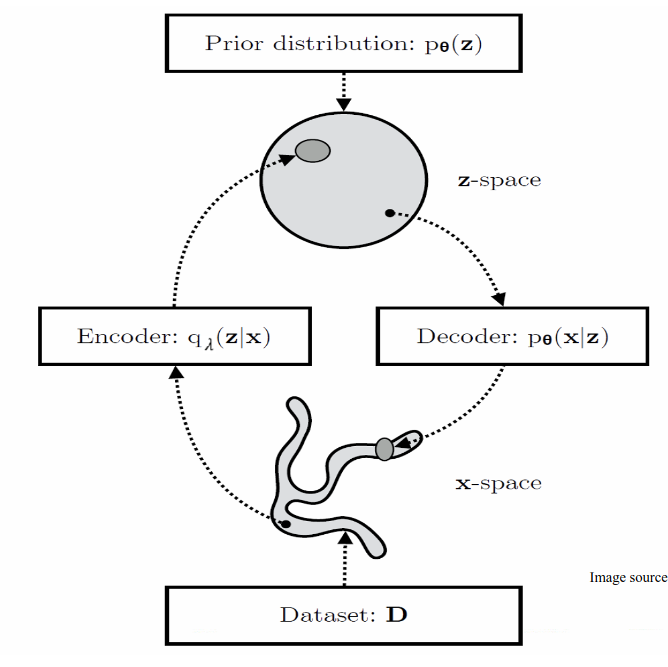
\includegraphics[scale=0.4]{img/08_VAE/VAE_framework.png}
    \end{center}
    If $q_{\lambda} = p_{\boldsymbol{\theta}}$, then the diagram commutes, i.e. $p(\mathbf{z}) p_{\boldsymbol{\theta}}(\mathbf{x} \mid \mathbf{z}) = p(\mathbf{x}) p_{\boldsymbol{\theta}}(\mathbf{z} \mid \mathbf{x}) = p_{\boldsymbol{\theta}} (\mathbf{x}, \mathbf{z})$. 
     
    \begin{example}
        If $\lambda = (\boldsymbol{\mu}, \boldsymbol{\sigma})$, where $\boldsymbol{\sigma}$ is just the vector representing variances of independent Gaussians, then we can use the neural network $\mathcal{E}$ to get 
        \[\lambda = \mathrm{EncoderNN}_{\phi} ( \mathbf{x}) = \mathcal{E}_{\phi} (\mathbf{x})\]
        In the example, $\lambda = (\boldsymbol{\mu}, \log \boldsymbol{\sigma}^2 )$ since we want to allow negative values, and $q_{\lambda} (\mathbf{z} \mid \mathbf{x}) = N(\mathbf{z} \mid \mathcal{E}_{\phi} (\mathbf{x})) = N(\mathbf{z} ; \, \boldsymbol{\mu} , \boldsymbol{\sigma}^2)$. 
    \end{example}

    Now, just like in RBMs and really any density estimation problem, our job is to maximize the log likelihood of the training set: 
    \[\sum_{t} \log p(\mathbf{x}^{(t)})\]

    In order to do this for this problem, we need a little fact to help us: 

    \begin{theorem}
    We have 
    \[KL \big( q_\lambda (\mathbf{z} \mid \mathbf{x}) \mid\mid p_{\boldsymbol{\theta}} (\mathbf{z} \mid \mathbf{x}) \big) = \mathbb{E}_{q_\lambda(\mathbf{z} \mid \mathbf{x})} [ \log q_{\lambda} (\mathbf{z} \mid \mathbf{x})] + \log p_{\boldsymbol{\theta}} (\mathbf{x}) - \mathbb{E}_{q_{\lambda} (\mathbf{z} \mid \mathbf{x})} [\log p_{\boldsymbol{\theta}} (\mathbf{x}, \mathbf{z})] \]
    and hence 
    \[\log p(\mathbf{x}) = KL \big( q_\lambda (\mathbf{z} \mid \mathbf{x}) \mid\mid p_{\boldsymbol{\theta}} (\mathbf{z} \mid \mathbf{x}) \big) + \mathbb{E}_{q_{\lambda} (\mathbf{z} \mid \mathbf{x})} [\log p_{\boldsymbol{\theta}} (\mathbf{x}, \mathbf{z})] - \mathbb{E}_{q_\lambda(\mathbf{z} \mid \mathbf{x})} [ \log q_{\lambda} (\mathbf{z} \mid \mathbf{x})]  \]
    \end{theorem}
    \begin{proof}
    TBD 
    \end{proof}

    So I have to maximize $\log  p(\mathbf{x})$ with what we have derived just now, but the KL divergence part is intractable, since $p_{\boldsymbol{\theta}} (\mathbf{z} \mid \mathbf{x})$ is intractable. That is the entire reason we chose $q_\lambda$! Using the fact that the KL divergence is always greater than or equal to $0$, we can drop the term and set a lower bound on the log likelihoods. This lower bound is called the \textbf{variational lower bound}.  
    \[\sum_{i=1}^N \log p_{\boldsymbol{\theta}} (\mathbf{x}^{(i)}) \geq \sum_{i=1}^N \mathbb{E}_{q_\lambda (\mathbf{z} \mid \mathbf{x}^{(i)})} [ \log p_{\boldsymbol{\theta}} (\mathbf{x}^{(i)}, \mathbf{z})] - \sum_{i=1}^N \mathbb{E}_{q_{\lambda} (\mathbf{z} \mid \mathbf{x}^{(i)})} [ \log q_{\lambda} (\mathbf{z} \mid \mathbf{x}^{(i)}) ] = \mathrm{ELBO}\]
    If we assume that no two data points share their latent variables with each other, then ELBO decomposes into the sum of
    \begin{align*} 
        \mathrm{ELBO} & = \sum_{i=1}^N \mathrm{ELBO}_i \\
                      & = \sum_{i=1}^N  \mathbb{E}_{q_\lambda (\mathbf{z} \mid \mathbf{x}^{(i)})} [\log p_{\boldsymbol{\theta}} (\mathbf{x}^{(i)}, \mathbf{z})] - \sum_{ i=1}^N \mathbb{E}_{q_\lambda (\mathbf{z} \mid \mathbf{x}^{(i)})}[ \log  q_{\lambda} (\mathbf{z} \mid \mathbf{x}^{(i)})] \\
                      & = \underbrace{\mathbb{E}_{q_\lambda (\mathbf{z} \mid \mathbf{x}^{(i)})} [\log p_{\boldsymbol{\theta}} (\mathbf{x}^{(i)} \mid \mathbf{z})]}_{\substack{\text{likelihood term} \\ \text{(reconstruction part)}}}- \underbrace{KL(q_{\lambda} (\mathbf{z} \mid \mathbf{x}^{(i)}) \mid\mid p(\mathbf{z}))}_{\substack{\text{closeness of encoding to } p(\mathbf{z}) \\ \text{(typically Gaussian)}}}
    \end{align*} 
    Typtically, $p(\mathbf{z})$ is chosen to be standard normal. This process is true regardless of it model classes $p_{\boldsymbol{\theta}} (\mathbf{x}^{(i)} \mid \mathbf{z})$ and $q_\lambda (\mathbf{z} \mid \mathbf{x})$ are given by deep neural nets or not. If it is a deep neural net, then it's called a deep latent model. 

    Now to compute gradients, let us denote the ELBO w.r.t. the decoder and encoder paramters as $\mathcal{L}_{\theta, \lambda}(\mathbf{x})$. Then, we can obtain the unbiased gradient w.r.t. $\theta$ as such: 
    \begin{align*} 
        \nabla_\theta \mathcal{L}_{\theta, \lambda} (\mathbf{x}) & = \nabla_\theta \big\{ \mathbb{E}_{q_\lambda (\mathbf{z} \mid \mathbf{x})} [ \log p_\theta (\mathbf{x}, \mathbf{z})] - \mathbb{E}_{q_\lambda (\mathbf{z} \mid \mathbf{x})} [\log q_{\lambda} (\mathbf{z} \mid \mathbf{x})] \} \\
                                                                 & = \mathbb{E}_{q_\lambda (\mathbf{z} \mid \mathbf{x})} \big[ \nabla_\theta \{ \log p_[\theta (\mathbf{x}, \mathbf{z}) - \log q_{\lambda} (\mathbf{z} \mid \mathbf{x}) \}  \big] \\
                                                                 & \approx \nabla_\theta \big\{ \log p_\theta(\mathbf{x}, \mathbf{z}) - \log q_\theta (\mathbf{z} \mid \mathbf{x}) \big\} \\
                                                                 & = \nabla_\theta \log p_\theta (\mathbf{x}, \mathbf{z}) 
    \end{align*}
    where the step with the $\approx$ just indicates that we approximate the expectation with a sample of size $1$ over some minibatch. However, taking the gradient w.r.t. $\lambda$ is more complicated since we cannot put the gradient in the expectation (since we are deriving and integrating w.r.t. $\lambda$).  Fortunately, for continuous RVs, the unbiased estimator of the gradient can be obtained through the \textbf{reparamaterization trick}, which is some change of variable. 

    \subsubsection{Reparameterization Trick} 

  \subsection{Variational Autoencoders} 

    In a VAE, the $q_{\lambda} (\mathbf{z} \mid \mathbf{x})$ is the encoder and the $p_{\boldsymbol{\theta}} (\mathbf{x} \mid \mathbf{z})$ is the decoder. 
    \begin{enumerate} 
        \item \textbf{Encoding Neural Network}: Upon observing $\mathbf{x}$, the neural network $\mathcal{E}$ outputs parameters $\lambda$. 
        \item \textbf{Decoding Neural Network}: Upon observing $\mathbf{z}$, the neural network $\mathcal{D}$ outputs parameters $\boldsymbol{\theta}$. 
    \end{enumerate} 

    We want to optimize $(\boldsymbol{\theta}, \lambda)$. To generate new samples, we just sample from $p(\mathbf{z})$ (usually standard Gaussian) and use the decoder to sample from $\mathbf{x}$.  

    This can be extended to deep layers. 

  \subsection{Conditional VAEs}

  \subsection{Importance Weighted Autoencoders}

